% Options for packages loaded elsewhere
\PassOptionsToPackage{unicode}{hyperref}
\PassOptionsToPackage{hyphens}{url}
\PassOptionsToPackage{dvipsnames,svgnames,x11names}{xcolor}
%
\documentclass[
  letterpaper,
  DIV=11,
  numbers=noendperiod]{scrartcl}

\usepackage{amsmath,amssymb}
\usepackage{iftex}
\ifPDFTeX
  \usepackage[T1]{fontenc}
  \usepackage[utf8]{inputenc}
  \usepackage{textcomp} % provide euro and other symbols
\else % if luatex or xetex
  \usepackage{unicode-math}
  \defaultfontfeatures{Scale=MatchLowercase}
  \defaultfontfeatures[\rmfamily]{Ligatures=TeX,Scale=1}
\fi
\usepackage{lmodern}
\ifPDFTeX\else  
    % xetex/luatex font selection
\fi
% Use upquote if available, for straight quotes in verbatim environments
\IfFileExists{upquote.sty}{\usepackage{upquote}}{}
\IfFileExists{microtype.sty}{% use microtype if available
  \usepackage[]{microtype}
  \UseMicrotypeSet[protrusion]{basicmath} % disable protrusion for tt fonts
}{}
\makeatletter
\@ifundefined{KOMAClassName}{% if non-KOMA class
  \IfFileExists{parskip.sty}{%
    \usepackage{parskip}
  }{% else
    \setlength{\parindent}{0pt}
    \setlength{\parskip}{6pt plus 2pt minus 1pt}}
}{% if KOMA class
  \KOMAoptions{parskip=half}}
\makeatother
\usepackage{xcolor}
\setlength{\emergencystretch}{3em} % prevent overfull lines
\setcounter{secnumdepth}{-\maxdimen} % remove section numbering
% Make \paragraph and \subparagraph free-standing
\makeatletter
\ifx\paragraph\undefined\else
  \let\oldparagraph\paragraph
  \renewcommand{\paragraph}{
    \@ifstar
      \xxxParagraphStar
      \xxxParagraphNoStar
  }
  \newcommand{\xxxParagraphStar}[1]{\oldparagraph*{#1}\mbox{}}
  \newcommand{\xxxParagraphNoStar}[1]{\oldparagraph{#1}\mbox{}}
\fi
\ifx\subparagraph\undefined\else
  \let\oldsubparagraph\subparagraph
  \renewcommand{\subparagraph}{
    \@ifstar
      \xxxSubParagraphStar
      \xxxSubParagraphNoStar
  }
  \newcommand{\xxxSubParagraphStar}[1]{\oldsubparagraph*{#1}\mbox{}}
  \newcommand{\xxxSubParagraphNoStar}[1]{\oldsubparagraph{#1}\mbox{}}
\fi
\makeatother

\usepackage{color}
\usepackage{fancyvrb}
\newcommand{\VerbBar}{|}
\newcommand{\VERB}{\Verb[commandchars=\\\{\}]}
\DefineVerbatimEnvironment{Highlighting}{Verbatim}{commandchars=\\\{\}}
% Add ',fontsize=\small' for more characters per line
\usepackage{framed}
\definecolor{shadecolor}{RGB}{241,243,245}
\newenvironment{Shaded}{\begin{snugshade}}{\end{snugshade}}
\newcommand{\AlertTok}[1]{\textcolor[rgb]{0.68,0.00,0.00}{#1}}
\newcommand{\AnnotationTok}[1]{\textcolor[rgb]{0.37,0.37,0.37}{#1}}
\newcommand{\AttributeTok}[1]{\textcolor[rgb]{0.40,0.45,0.13}{#1}}
\newcommand{\BaseNTok}[1]{\textcolor[rgb]{0.68,0.00,0.00}{#1}}
\newcommand{\BuiltInTok}[1]{\textcolor[rgb]{0.00,0.23,0.31}{#1}}
\newcommand{\CharTok}[1]{\textcolor[rgb]{0.13,0.47,0.30}{#1}}
\newcommand{\CommentTok}[1]{\textcolor[rgb]{0.37,0.37,0.37}{#1}}
\newcommand{\CommentVarTok}[1]{\textcolor[rgb]{0.37,0.37,0.37}{\textit{#1}}}
\newcommand{\ConstantTok}[1]{\textcolor[rgb]{0.56,0.35,0.01}{#1}}
\newcommand{\ControlFlowTok}[1]{\textcolor[rgb]{0.00,0.23,0.31}{\textbf{#1}}}
\newcommand{\DataTypeTok}[1]{\textcolor[rgb]{0.68,0.00,0.00}{#1}}
\newcommand{\DecValTok}[1]{\textcolor[rgb]{0.68,0.00,0.00}{#1}}
\newcommand{\DocumentationTok}[1]{\textcolor[rgb]{0.37,0.37,0.37}{\textit{#1}}}
\newcommand{\ErrorTok}[1]{\textcolor[rgb]{0.68,0.00,0.00}{#1}}
\newcommand{\ExtensionTok}[1]{\textcolor[rgb]{0.00,0.23,0.31}{#1}}
\newcommand{\FloatTok}[1]{\textcolor[rgb]{0.68,0.00,0.00}{#1}}
\newcommand{\FunctionTok}[1]{\textcolor[rgb]{0.28,0.35,0.67}{#1}}
\newcommand{\ImportTok}[1]{\textcolor[rgb]{0.00,0.46,0.62}{#1}}
\newcommand{\InformationTok}[1]{\textcolor[rgb]{0.37,0.37,0.37}{#1}}
\newcommand{\KeywordTok}[1]{\textcolor[rgb]{0.00,0.23,0.31}{\textbf{#1}}}
\newcommand{\NormalTok}[1]{\textcolor[rgb]{0.00,0.23,0.31}{#1}}
\newcommand{\OperatorTok}[1]{\textcolor[rgb]{0.37,0.37,0.37}{#1}}
\newcommand{\OtherTok}[1]{\textcolor[rgb]{0.00,0.23,0.31}{#1}}
\newcommand{\PreprocessorTok}[1]{\textcolor[rgb]{0.68,0.00,0.00}{#1}}
\newcommand{\RegionMarkerTok}[1]{\textcolor[rgb]{0.00,0.23,0.31}{#1}}
\newcommand{\SpecialCharTok}[1]{\textcolor[rgb]{0.37,0.37,0.37}{#1}}
\newcommand{\SpecialStringTok}[1]{\textcolor[rgb]{0.13,0.47,0.30}{#1}}
\newcommand{\StringTok}[1]{\textcolor[rgb]{0.13,0.47,0.30}{#1}}
\newcommand{\VariableTok}[1]{\textcolor[rgb]{0.07,0.07,0.07}{#1}}
\newcommand{\VerbatimStringTok}[1]{\textcolor[rgb]{0.13,0.47,0.30}{#1}}
\newcommand{\WarningTok}[1]{\textcolor[rgb]{0.37,0.37,0.37}{\textit{#1}}}

\providecommand{\tightlist}{%
  \setlength{\itemsep}{0pt}\setlength{\parskip}{0pt}}\usepackage{longtable,booktabs,array}
\usepackage{calc} % for calculating minipage widths
% Correct order of tables after \paragraph or \subparagraph
\usepackage{etoolbox}
\makeatletter
\patchcmd\longtable{\par}{\if@noskipsec\mbox{}\fi\par}{}{}
\makeatother
% Allow footnotes in longtable head/foot
\IfFileExists{footnotehyper.sty}{\usepackage{footnotehyper}}{\usepackage{footnote}}
\makesavenoteenv{longtable}
\usepackage{graphicx}
\makeatletter
\newsavebox\pandoc@box
\newcommand*\pandocbounded[1]{% scales image to fit in text height/width
  \sbox\pandoc@box{#1}%
  \Gscale@div\@tempa{\textheight}{\dimexpr\ht\pandoc@box+\dp\pandoc@box\relax}%
  \Gscale@div\@tempb{\linewidth}{\wd\pandoc@box}%
  \ifdim\@tempb\p@<\@tempa\p@\let\@tempa\@tempb\fi% select the smaller of both
  \ifdim\@tempa\p@<\p@\scalebox{\@tempa}{\usebox\pandoc@box}%
  \else\usebox{\pandoc@box}%
  \fi%
}
% Set default figure placement to htbp
\def\fps@figure{htbp}
\makeatother

\usepackage[margin=0.7in]{geometry}
\usepackage{fvextra}
\DefineVerbatimEnvironment{Highlighting}{Verbatim}{breaklines,commandchars=\\\{\}}
\KOMAoption{captions}{tableheading}
\makeatletter
\@ifpackageloaded{caption}{}{\usepackage{caption}}
\AtBeginDocument{%
\ifdefined\contentsname
  \renewcommand*\contentsname{Table of contents}
\else
  \newcommand\contentsname{Table of contents}
\fi
\ifdefined\listfigurename
  \renewcommand*\listfigurename{List of Figures}
\else
  \newcommand\listfigurename{List of Figures}
\fi
\ifdefined\listtablename
  \renewcommand*\listtablename{List of Tables}
\else
  \newcommand\listtablename{List of Tables}
\fi
\ifdefined\figurename
  \renewcommand*\figurename{Figure}
\else
  \newcommand\figurename{Figure}
\fi
\ifdefined\tablename
  \renewcommand*\tablename{Table}
\else
  \newcommand\tablename{Table}
\fi
}
\@ifpackageloaded{float}{}{\usepackage{float}}
\floatstyle{ruled}
\@ifundefined{c@chapter}{\newfloat{codelisting}{h}{lop}}{\newfloat{codelisting}{h}{lop}[chapter]}
\floatname{codelisting}{Listing}
\newcommand*\listoflistings{\listof{codelisting}{List of Listings}}
\makeatother
\makeatletter
\makeatother
\makeatletter
\@ifpackageloaded{caption}{}{\usepackage{caption}}
\@ifpackageloaded{subcaption}{}{\usepackage{subcaption}}
\makeatother

\usepackage{bookmark}

\IfFileExists{xurl.sty}{\usepackage{xurl}}{} % add URL line breaks if available
\urlstyle{same} % disable monospaced font for URLs
\hypersetup{
  pdftitle={problem set IV},
  colorlinks=true,
  linkcolor={blue},
  filecolor={Maroon},
  citecolor={Blue},
  urlcolor={Blue},
  pdfcreator={LaTeX via pandoc}}


\title{problem set IV}
\author{Jenny Zhong \& Summer Negahdar}
\date{}

\begin{document}
\maketitle

\RecustomVerbatimEnvironment{verbatim}{Verbatim}{
  showspaces = false,
  showtabs = false,
  breaksymbolleft={},
  breaklines
}


``This submission is our work alone and complies with the 30538
integrity policy.'' Add your initials to indicate your agreement:
\textbf{SN} \textbf{JZ}

``I have uploaded the names of anyone else other than my partner and I
worked with on the problem set
\textbf{\href{https://docs.google.com/forms/d/185usrCREQaUbvAXpWhChkjghdGgmAZXA3lPWpXLLsts/edit}{here}}''
(1 point) Late coins used this pset: **1 this pset** Late coins left
after submission: **\textbackslash0** Knit your \texttt{ps4.qmd} to an
PDF file to make \texttt{ps4.pdf},

\subsection{Download and explore the Provider of Services (POS)
file}\label{download-and-explore-the-provider-of-services-pos-file}

\begin{enumerate}
\def\labelenumi{\arabic{enumi}.}
\tightlist
\item
  PRVDR\_CTGRY\_SBTYP\_CD: Provider subtype for reporting categories.
\end{enumerate}

PRVDR\_CTGRY\_CD: Provider type in Medicare/Medicaid programs.

PGM\_TRMNTN\_CD: Provider's current termination status code.

TRMNTN\_EXPRTN\_DT: Provider termination or certificate expiration date.

FAC\_NAME: Certified facility or hospital's official name.

ZIP\_CD: Provider's five-digit ZIP code.

CHOW\_CNT: Number of provider ownership changes.

CHOW\_DT: Date of latest ownership change.

CITY\_NAME: Provider's physical location city.

PRVDR\_NUM: CMS-certified provider's unique identification number.

\begin{enumerate}
\def\labelenumi{\arabic{enumi}.}
\setcounter{enumi}{1}
\tightlist
\item
\end{enumerate}

\begin{Shaded}
\begin{Highlighting}[]
\ImportTok{import}\NormalTok{ pandas }\ImportTok{as}\NormalTok{ pd}
\ImportTok{import}\NormalTok{ geopandas }\ImportTok{as}\NormalTok{ gpd}
\ImportTok{import}\NormalTok{ shapely}
\ImportTok{import}\NormalTok{ altair }\ImportTok{as}\NormalTok{ alt}
\ImportTok{import}\NormalTok{ sys}
\ImportTok{import}\NormalTok{ pyproj}
\ImportTok{import}\NormalTok{ os}
\ImportTok{from}\NormalTok{ pyproj }\ImportTok{import}\NormalTok{ CRS, Transformer}

\NormalTok{file\_path }\OperatorTok{=} \StringTok{\textquotesingle{}/Users/samarnegahdar/Desktop/untitled folder/problem{-}set{-}4{-}summer{-}jenny\textquotesingle{}}

\NormalTok{pos2016 }\OperatorTok{=}\NormalTok{ pd.read\_csv(}\StringTok{\textquotesingle{}pos2016.csv\textquotesingle{}}\NormalTok{)}

\NormalTok{pos2016.head(}\DecValTok{3}\NormalTok{)}

\CommentTok{\#converting to string}
\NormalTok{pos2016[}\StringTok{\textquotesingle{}PRVDR\_CTGRY\_SBTYP\_CD\textquotesingle{}}\NormalTok{] }\OperatorTok{=}\NormalTok{ pos2016[}\StringTok{\textquotesingle{}PRVDR\_CTGRY\_SBTYP\_CD\textquotesingle{}}\NormalTok{].astype(}\BuiltInTok{str}\NormalTok{).}\BuiltInTok{str}\NormalTok{.zfill(}\DecValTok{2}\NormalTok{)}

\NormalTok{pos2016[}\StringTok{\textquotesingle{}PRVDR\_CTGRY\_CD\textquotesingle{}}\NormalTok{] }\OperatorTok{=}\NormalTok{ pos2016[}\StringTok{\textquotesingle{}PRVDR\_CTGRY\_CD\textquotesingle{}}\NormalTok{].astype(}\BuiltInTok{str}\NormalTok{).}\BuiltInTok{str}\NormalTok{.zfill(}\DecValTok{2}\NormalTok{)}
\NormalTok{pos2016.head(}\DecValTok{3}\NormalTok{)}

\NormalTok{st\_hospitals2016 }\OperatorTok{=}\NormalTok{ pos2016[(pos2016[}\StringTok{\textquotesingle{}PRVDR\_CTGRY\_SBTYP\_CD\textquotesingle{}}\NormalTok{] }\OperatorTok{==} \StringTok{\textquotesingle{}1.0\textquotesingle{}}\NormalTok{) }\OperatorTok{\&}\NormalTok{ (pos2016[}\StringTok{\textquotesingle{}PRVDR\_CTGRY\_CD\textquotesingle{}}\NormalTok{] }\OperatorTok{==} \StringTok{\textquotesingle{}01\textquotesingle{}}\NormalTok{)]}

\BuiltInTok{print}\NormalTok{(st\_hospitals2016.head(}\DecValTok{3}\NormalTok{))}
\NormalTok{st\_hospitals2016.shape}
\end{Highlighting}
\end{Shaded}

\begin{verbatim}
  PRVDR_CTGRY_SBTYP_CD PRVDR_CTGRY_CD  CHOW_CNT  CHOW_DT   CITY_NAME  \
0                  1.0             01         1      NaN      DOTHAN   
1                  1.0             01         0      NaN  BRIDGEPORT   
2                  1.0             01         0      NaN        BOAZ   

                           FAC_NAME PRVDR_NUM  PGM_TRMNTN_CD  \
0  SOUTHEAST ALABAMA MEDICAL CENTER    010001              0   
1            NORTH JACKSON HOSPITAL    010004              1   
2     MARSHALL MEDICAL CENTER SOUTH    010005              0   

   TRMNTN_EXPRTN_DT   ZIP_CD  
0               NaN  36301.0  
1        20010831.0  35740.0  
2               NaN  35957.0  
\end{verbatim}

\begin{verbatim}
(7245, 10)
\end{verbatim}

\begin{enumerate}
\def\labelenumi{\alph{enumi}.}
\tightlist
\item
  7,245 hospitals are reported in this data.
\item
  Compared to sources that provide counts of short-term hospitals in the
  US, such as the Kaiser Family Foundation, we know that there were
  nearly 5,000 short term, acute care hospitals in the US in recent
  years (half of which are rural and half urban). This could be higher
  than the reported number because of definition differences, for
  example the dataset could define short-term hospitals different to the
  Kaiser Family Foundation's definition. adding the year 2016
\end{enumerate}

\begin{Shaded}
\begin{Highlighting}[]
\NormalTok{st\_hospitals2016.loc[:, }\StringTok{\textquotesingle{}YEAR\textquotesingle{}}\NormalTok{] }\OperatorTok{=} \DecValTok{2016}
\BuiltInTok{print}\NormalTok{(st\_hospitals2016.head(}\DecValTok{3}\NormalTok{))}
\end{Highlighting}
\end{Shaded}

\begin{verbatim}
  PRVDR_CTGRY_SBTYP_CD PRVDR_CTGRY_CD  CHOW_CNT  CHOW_DT   CITY_NAME  \
0                  1.0             01         1      NaN      DOTHAN   
1                  1.0             01         0      NaN  BRIDGEPORT   
2                  1.0             01         0      NaN        BOAZ   

                           FAC_NAME PRVDR_NUM  PGM_TRMNTN_CD  \
0  SOUTHEAST ALABAMA MEDICAL CENTER    010001              0   
1            NORTH JACKSON HOSPITAL    010004              1   
2     MARSHALL MEDICAL CENTER SOUTH    010005              0   

   TRMNTN_EXPRTN_DT   ZIP_CD  YEAR  
0               NaN  36301.0  2016  
1        20010831.0  35740.0  2016  
2               NaN  35957.0  2016  
\end{verbatim}

\begin{verbatim}
/var/folders/j5/rv933w1173s068kbzq0kp2xh0000gn/T/ipykernel_9517/3669868829.py:1: SettingWithCopyWarning: 
A value is trying to be set on a copy of a slice from a DataFrame.
Try using .loc[row_indexer,col_indexer] = value instead

See the caveats in the documentation: https://pandas.pydata.org/pandas-docs/stable/user_guide/indexing.html#returning-a-view-versus-a-copy
  st_hospitals2016.loc[:, 'YEAR'] = 2016
\end{verbatim}

\begin{enumerate}
\def\labelenumi{\arabic{enumi}.}
\setcounter{enumi}{2}
\tightlist
\item
  for 2017:
\end{enumerate}

\begin{Shaded}
\begin{Highlighting}[]
\CommentTok{\#importing pos2017}
\NormalTok{pos2017 }\OperatorTok{=}\NormalTok{ pd.read\_csv(}\StringTok{"pos2017.csv"}\NormalTok{, encoding}\OperatorTok{=}\StringTok{\textquotesingle{}latin1\textquotesingle{}}\NormalTok{)}
\CommentTok{\#converting to string}
\NormalTok{pos2017[}\StringTok{\textquotesingle{}PRVDR\_CTGRY\_SBTYP\_CD\textquotesingle{}}\NormalTok{] }\OperatorTok{=}\NormalTok{ pos2017[}\StringTok{\textquotesingle{}PRVDR\_CTGRY\_SBTYP\_CD\textquotesingle{}}\NormalTok{].astype(}\BuiltInTok{str}\NormalTok{).}\BuiltInTok{str}\NormalTok{.zfill(}\DecValTok{2}\NormalTok{)}

\NormalTok{pos2017[}\StringTok{\textquotesingle{}PRVDR\_CTGRY\_CD\textquotesingle{}}\NormalTok{] }\OperatorTok{=}\NormalTok{ pos2017[}\StringTok{\textquotesingle{}PRVDR\_CTGRY\_CD\textquotesingle{}}\NormalTok{].astype(}\BuiltInTok{str}\NormalTok{).}\BuiltInTok{str}\NormalTok{.zfill(}\DecValTok{2}\NormalTok{) }\CommentTok{\#\#filling numbers with a zero before integer}
\NormalTok{pos2017.head(}\DecValTok{3}\NormalTok{)}
\CommentTok{\#then focusing on short term hospitals }
\NormalTok{st\_hospitals2017 }\OperatorTok{=}\NormalTok{ pos2017[(pos2017[}\StringTok{\textquotesingle{}PRVDR\_CTGRY\_SBTYP\_CD\textquotesingle{}}\NormalTok{] }\OperatorTok{==} \StringTok{\textquotesingle{}1.0\textquotesingle{}}\NormalTok{) }\OperatorTok{\&}\NormalTok{ (pos2017[}\StringTok{\textquotesingle{}PRVDR\_CTGRY\_CD\textquotesingle{}}\NormalTok{] }\OperatorTok{==} \StringTok{\textquotesingle{}01\textquotesingle{}}\NormalTok{)]}

\BuiltInTok{print}\NormalTok{(st\_hospitals2017.head(}\DecValTok{3}\NormalTok{))}
\BuiltInTok{print}\NormalTok{(st\_hospitals2017.tail(}\DecValTok{3}\NormalTok{))}
\NormalTok{st\_hospitals2017.shape}
\end{Highlighting}
\end{Shaded}

\begin{verbatim}
  PRVDR_CTGRY_SBTYP_CD PRVDR_CTGRY_CD  CHOW_CNT  CHOW_DT   CITY_NAME  \
0                  1.0             01         1      NaN      DOTHAN   
1                  1.0             01         0      NaN  BRIDGEPORT   
2                  1.0             01         0      NaN        BOAZ   

                           FAC_NAME PRVDR_NUM  PGM_TRMNTN_CD  \
0  SOUTHEAST ALABAMA MEDICAL CENTER    010001              0   
1            NORTH JACKSON HOSPITAL    010004              1   
2     MARSHALL MEDICAL CENTER SOUTH    010005              0   

   TRMNTN_EXPRTN_DT   ZIP_CD  
0               NaN  36301.0  
1        20010831.0  35740.0  
2               NaN  35957.0  
       PRVDR_CTGRY_SBTYP_CD PRVDR_CTGRY_CD  CHOW_CNT  CHOW_DT      CITY_NAME  \
135473                  1.0             01         0      NaN        EL PASO   
135474                  1.0             01         0      NaN          HURST   
135475                  1.0             01         0      NaN  THE WOODLANDS   

                                                FAC_NAME PRVDR_NUM  \
135473  THE HOSPITALS OF PROVIDENCE TRANSMOUNTAIN CAMPUS    670120   
135474                     SAINT CAMILLUS MEDICAL CENTER    670121   
135475          HOUSTON METHODIST THE WOODLANDS HOSPITAL    670122   

        PGM_TRMNTN_CD  TRMNTN_EXPRTN_DT   ZIP_CD  
135473              0               NaN  79911.0  
135474              0               NaN  76054.0  
135475              0               NaN  77385.0  
\end{verbatim}

\begin{verbatim}
(7260, 10)
\end{verbatim}

Adding the 2017 column

\begin{Shaded}
\begin{Highlighting}[]
\NormalTok{st\_hospitals2017.loc[:, }\StringTok{\textquotesingle{}YEAR\textquotesingle{}}\NormalTok{] }\OperatorTok{=} \DecValTok{2017}

\BuiltInTok{print}\NormalTok{(st\_hospitals2017.head(}\DecValTok{3}\NormalTok{))}
\end{Highlighting}
\end{Shaded}

\begin{verbatim}
  PRVDR_CTGRY_SBTYP_CD PRVDR_CTGRY_CD  CHOW_CNT  CHOW_DT   CITY_NAME  \
0                  1.0             01         1      NaN      DOTHAN   
1                  1.0             01         0      NaN  BRIDGEPORT   
2                  1.0             01         0      NaN        BOAZ   

                           FAC_NAME PRVDR_NUM  PGM_TRMNTN_CD  \
0  SOUTHEAST ALABAMA MEDICAL CENTER    010001              0   
1            NORTH JACKSON HOSPITAL    010004              1   
2     MARSHALL MEDICAL CENTER SOUTH    010005              0   

   TRMNTN_EXPRTN_DT   ZIP_CD  YEAR  
0               NaN  36301.0  2017  
1        20010831.0  35740.0  2017  
2               NaN  35957.0  2017  
\end{verbatim}

\begin{verbatim}
/var/folders/j5/rv933w1173s068kbzq0kp2xh0000gn/T/ipykernel_9517/196776328.py:1: SettingWithCopyWarning: 
A value is trying to be set on a copy of a slice from a DataFrame.
Try using .loc[row_indexer,col_indexer] = value instead

See the caveats in the documentation: https://pandas.pydata.org/pandas-docs/stable/user_guide/indexing.html#returning-a-view-versus-a-copy
  st_hospitals2017.loc[:, 'YEAR'] = 2017
\end{verbatim}

for 2018:

\begin{Shaded}
\begin{Highlighting}[]
\CommentTok{\#importing pos2018}
\NormalTok{pos2018 }\OperatorTok{=}\NormalTok{ pd.read\_csv(}\StringTok{\textquotesingle{}pos2018.csv\textquotesingle{}}\NormalTok{, encoding}\OperatorTok{=}\StringTok{\textquotesingle{}latin1\textquotesingle{}}\NormalTok{)}
\CommentTok{\#converting to string}
\NormalTok{pos2018[}\StringTok{\textquotesingle{}PRVDR\_CTGRY\_SBTYP\_CD\textquotesingle{}}\NormalTok{] }\OperatorTok{=}\NormalTok{ pos2018[}\StringTok{\textquotesingle{}PRVDR\_CTGRY\_SBTYP\_CD\textquotesingle{}}\NormalTok{].astype(}\BuiltInTok{str}\NormalTok{).}\BuiltInTok{str}\NormalTok{.zfill(}\DecValTok{2}\NormalTok{)}

\NormalTok{pos2018[}\StringTok{\textquotesingle{}PRVDR\_CTGRY\_CD\textquotesingle{}}\NormalTok{] }\OperatorTok{=}\NormalTok{ pos2018[}\StringTok{\textquotesingle{}PRVDR\_CTGRY\_CD\textquotesingle{}}\NormalTok{].astype(}\BuiltInTok{str}\NormalTok{).}\BuiltInTok{str}\NormalTok{.zfill(}\DecValTok{2}\NormalTok{)}
\NormalTok{pos2018.head(}\DecValTok{3}\NormalTok{)}
\CommentTok{\#then focus on st hospitals }
\NormalTok{st\_hospitals2018 }\OperatorTok{=}\NormalTok{ pos2018[(pos2018[}\StringTok{\textquotesingle{}PRVDR\_CTGRY\_SBTYP\_CD\textquotesingle{}}\NormalTok{] }\OperatorTok{==} \StringTok{\textquotesingle{}1.0\textquotesingle{}}\NormalTok{) }\OperatorTok{\&}\NormalTok{ (pos2018[}\StringTok{\textquotesingle{}PRVDR\_CTGRY\_CD\textquotesingle{}}\NormalTok{] }\OperatorTok{==} \StringTok{\textquotesingle{}01\textquotesingle{}}\NormalTok{)]}

\BuiltInTok{print}\NormalTok{(st\_hospitals2018.head(}\DecValTok{3}\NormalTok{))}
\BuiltInTok{print}\NormalTok{(st\_hospitals2018.tail(}\DecValTok{3}\NormalTok{))}
\NormalTok{st\_hospitals2018.shape}
\end{Highlighting}
\end{Shaded}

\begin{verbatim}
  PRVDR_CTGRY_SBTYP_CD PRVDR_CTGRY_CD  CHOW_CNT  CHOW_DT   CITY_NAME  \
0                  1.0             01         1      NaN      DOTHAN   
1                  1.0             01         0      NaN  BRIDGEPORT   
2                  1.0             01         0      NaN        BOAZ   

                           FAC_NAME PRVDR_NUM  PGM_TRMNTN_CD  \
0  SOUTHEAST ALABAMA MEDICAL CENTER    010001              0   
1            NORTH JACKSON HOSPITAL    010004              1   
2     MARSHALL MEDICAL CENTER SOUTH    010005              0   

   TRMNTN_EXPRTN_DT   ZIP_CD  
0               NaN  36301.0  
1        20010831.0  35740.0  
2               NaN  35957.0  
       PRVDR_CTGRY_SBTYP_CD PRVDR_CTGRY_CD  CHOW_CNT  CHOW_DT     CITY_NAME  \
137569                  1.0             01         0      NaN  HORIZON CITY   
137570                  1.0             01         0      NaN   SAN ANTONIO   
137571                  1.0             01         0      NaN      CROCKETT   

                                               FAC_NAME PRVDR_NUM  \
137569  THE HOSPITALS OF PROVIDENCE HORIZON CITY CAMPUS    670124   
137570              TEXAS CENTER FOR INFECTIOUS DISEASE    670125   
137571                          CROCKETT MEDICAL CENTER    670126   

        PGM_TRMNTN_CD  TRMNTN_EXPRTN_DT   ZIP_CD  
137569              0               NaN  79928.0  
137570              0               NaN  78223.0  
137571              0               NaN  75835.0  
\end{verbatim}

\begin{verbatim}
(7277, 10)
\end{verbatim}

Adding the 2018 column

\begin{Shaded}
\begin{Highlighting}[]
\CommentTok{\#column had to be extended}
\NormalTok{st\_hospitals2018.loc[:, }\StringTok{\textquotesingle{}YEAR\textquotesingle{}}\NormalTok{] }\OperatorTok{=} \DecValTok{2018}

\BuiltInTok{print}\NormalTok{(st\_hospitals2018.head(}\DecValTok{3}\NormalTok{))}
\end{Highlighting}
\end{Shaded}

\begin{verbatim}
  PRVDR_CTGRY_SBTYP_CD PRVDR_CTGRY_CD  CHOW_CNT  CHOW_DT   CITY_NAME  \
0                  1.0             01         1      NaN      DOTHAN   
1                  1.0             01         0      NaN  BRIDGEPORT   
2                  1.0             01         0      NaN        BOAZ   

                           FAC_NAME PRVDR_NUM  PGM_TRMNTN_CD  \
0  SOUTHEAST ALABAMA MEDICAL CENTER    010001              0   
1            NORTH JACKSON HOSPITAL    010004              1   
2     MARSHALL MEDICAL CENTER SOUTH    010005              0   

   TRMNTN_EXPRTN_DT   ZIP_CD  YEAR  
0               NaN  36301.0  2018  
1        20010831.0  35740.0  2018  
2               NaN  35957.0  2018  
\end{verbatim}

\begin{verbatim}
/var/folders/j5/rv933w1173s068kbzq0kp2xh0000gn/T/ipykernel_9517/471435673.py:2: SettingWithCopyWarning: 
A value is trying to be set on a copy of a slice from a DataFrame.
Try using .loc[row_indexer,col_indexer] = value instead

See the caveats in the documentation: https://pandas.pydata.org/pandas-docs/stable/user_guide/indexing.html#returning-a-view-versus-a-copy
  st_hospitals2018.loc[:, 'YEAR'] = 2018
\end{verbatim}

for 2019:

\begin{Shaded}
\begin{Highlighting}[]
\CommentTok{\#importing pos2019}
\NormalTok{pos2019 }\OperatorTok{=}\NormalTok{ pd.read\_csv(}\StringTok{\textquotesingle{}pos2019.csv\textquotesingle{}}\NormalTok{, encoding}\OperatorTok{=}\StringTok{\textquotesingle{}latin1\textquotesingle{}}\NormalTok{)}

\CommentTok{\#converting to string}
\NormalTok{pos2019[}\StringTok{\textquotesingle{}PRVDR\_CTGRY\_SBTYP\_CD\textquotesingle{}}\NormalTok{] }\OperatorTok{=}\NormalTok{ pos2019[}\StringTok{\textquotesingle{}PRVDR\_CTGRY\_SBTYP\_CD\textquotesingle{}}\NormalTok{].astype(}\BuiltInTok{str}\NormalTok{).}\BuiltInTok{str}\NormalTok{.zfill(}\DecValTok{2}\NormalTok{)}

\NormalTok{pos2019[}\StringTok{\textquotesingle{}PRVDR\_CTGRY\_CD\textquotesingle{}}\NormalTok{] }\OperatorTok{=}\NormalTok{ pos2019[}\StringTok{\textquotesingle{}PRVDR\_CTGRY\_CD\textquotesingle{}}\NormalTok{].astype(}\BuiltInTok{str}\NormalTok{).}\BuiltInTok{str}\NormalTok{.zfill(}\DecValTok{2}\NormalTok{)}
\NormalTok{pos2019.head(}\DecValTok{3}\NormalTok{)}
\CommentTok{\#then focus on st hospitals }
\NormalTok{st\_hospitals2019 }\OperatorTok{=}\NormalTok{ pos2019[(pos2019[}\StringTok{\textquotesingle{}PRVDR\_CTGRY\_SBTYP\_CD\textquotesingle{}}\NormalTok{] }\OperatorTok{==} \StringTok{\textquotesingle{}1.0\textquotesingle{}}\NormalTok{) }\OperatorTok{\&}\NormalTok{ (pos2019[}\StringTok{\textquotesingle{}PRVDR\_CTGRY\_CD\textquotesingle{}}\NormalTok{] }\OperatorTok{==} \StringTok{\textquotesingle{}01\textquotesingle{}}\NormalTok{)]}

\BuiltInTok{print}\NormalTok{(st\_hospitals2019.head(}\DecValTok{3}\NormalTok{))}
\BuiltInTok{print}\NormalTok{(st\_hospitals2019.tail(}\DecValTok{3}\NormalTok{))}
\NormalTok{st\_hospitals2019.shape}
\end{Highlighting}
\end{Shaded}

\begin{verbatim}
  PRVDR_CTGRY_SBTYP_CD PRVDR_CTGRY_CD  CHOW_CNT  CHOW_DT   CITY_NAME  \
0                  1.0             01         1      NaN      DOTHAN   
1                  1.0             01         0      NaN  BRIDGEPORT   
2                  1.0             01         0      NaN        BOAZ   

                                FAC_NAME PRVDR_NUM  PGM_TRMNTN_CD  \
0       SOUTHEAST ALABAMA MEDICAL CENTER    010001              0   
1                 NORTH JACKSON HOSPITAL    010004              1   
2  MARSHALL MEDICAL CENTERS SOUTH CAMPUS    010005              0   

   TRMNTN_EXPRTN_DT   ZIP_CD  
0               NaN  36301.0  
1        20010831.0  35740.0  
2               NaN  35957.0  
       PRVDR_CTGRY_SBTYP_CD PRVDR_CTGRY_CD  CHOW_CNT  CHOW_DT     CITY_NAME  \
139516                  1.0             01         0      NaN  PFLUGERVILLE   
139517                  1.0             01         0      NaN       HOUSTON   
139518                  1.0             01         0      NaN   SAN ANTONIO   

                                                 FAC_NAME PRVDR_NUM  \
139516  BAYLOR SCOTT & WHITE MEDICAL CENTER ˜ PFLUGERV...    670128   
139517                               THE HEIGHTS HOSPITAL    670129   
139518                                SOUTHCROSS HOSPITAL    670130   

        PGM_TRMNTN_CD  TRMNTN_EXPRTN_DT   ZIP_CD  
139516              0               NaN  78660.0  
139517              0               NaN  77008.0  
139518              0               NaN  78222.0  
\end{verbatim}

\begin{verbatim}
(7303, 10)
\end{verbatim}

Adding the 2019 column

\begin{Shaded}
\begin{Highlighting}[]
\NormalTok{st\_hospitals2019.loc[:, }\StringTok{\textquotesingle{}YEAR\textquotesingle{}}\NormalTok{] }\OperatorTok{=} \DecValTok{2019}

\BuiltInTok{print}\NormalTok{(st\_hospitals2019.head(}\DecValTok{3}\NormalTok{))}
\end{Highlighting}
\end{Shaded}

\begin{verbatim}
  PRVDR_CTGRY_SBTYP_CD PRVDR_CTGRY_CD  CHOW_CNT  CHOW_DT   CITY_NAME  \
0                  1.0             01         1      NaN      DOTHAN   
1                  1.0             01         0      NaN  BRIDGEPORT   
2                  1.0             01         0      NaN        BOAZ   

                                FAC_NAME PRVDR_NUM  PGM_TRMNTN_CD  \
0       SOUTHEAST ALABAMA MEDICAL CENTER    010001              0   
1                 NORTH JACKSON HOSPITAL    010004              1   
2  MARSHALL MEDICAL CENTERS SOUTH CAMPUS    010005              0   

   TRMNTN_EXPRTN_DT   ZIP_CD  YEAR  
0               NaN  36301.0  2019  
1        20010831.0  35740.0  2019  
2               NaN  35957.0  2019  
\end{verbatim}

\begin{verbatim}
/var/folders/j5/rv933w1173s068kbzq0kp2xh0000gn/T/ipykernel_9517/1295493316.py:1: SettingWithCopyWarning: 
A value is trying to be set on a copy of a slice from a DataFrame.
Try using .loc[row_indexer,col_indexer] = value instead

See the caveats in the documentation: https://pandas.pydata.org/pandas-docs/stable/user_guide/indexing.html#returning-a-view-versus-a-copy
  st_hospitals2019.loc[:, 'YEAR'] = 2019
\end{verbatim}

\textbf{Appending them together}

\begin{Shaded}
\begin{Highlighting}[]
\NormalTok{all\_years\_data }\OperatorTok{=}\NormalTok{ pd.concat([st\_hospitals2016, st\_hospitals2017, st\_hospitals2018, st\_hospitals2019], ignore\_index}\OperatorTok{=}\VariableTok{True}\NormalTok{)}

\BuiltInTok{print}\NormalTok{(all\_years\_data.head(}\DecValTok{3}\NormalTok{))}
\NormalTok{all\_years\_data.shape}
\end{Highlighting}
\end{Shaded}

\begin{verbatim}
  PRVDR_CTGRY_SBTYP_CD PRVDR_CTGRY_CD  CHOW_CNT  CHOW_DT   CITY_NAME  \
0                  1.0             01         1      NaN      DOTHAN   
1                  1.0             01         0      NaN  BRIDGEPORT   
2                  1.0             01         0      NaN        BOAZ   

                           FAC_NAME PRVDR_NUM  PGM_TRMNTN_CD  \
0  SOUTHEAST ALABAMA MEDICAL CENTER    010001              0   
1            NORTH JACKSON HOSPITAL    010004              1   
2     MARSHALL MEDICAL CENTER SOUTH    010005              0   

   TRMNTN_EXPRTN_DT   ZIP_CD  YEAR  
0               NaN  36301.0  2016  
1        20010831.0  35740.0  2016  
2               NaN  35957.0  2016  
\end{verbatim}

\begin{verbatim}
(29085, 11)
\end{verbatim}

\textbf{Plotting by observations}

\begin{Shaded}
\begin{Highlighting}[]
\NormalTok{observations\_by\_year }\OperatorTok{=}\NormalTok{ all\_years\_data.groupby(}\StringTok{\textquotesingle{}YEAR\textquotesingle{}}\NormalTok{).size().reset\_index(name}\OperatorTok{=}\StringTok{\textquotesingle{}count\textquotesingle{}}\NormalTok{)}

\NormalTok{chart13 }\OperatorTok{=}\NormalTok{ alt.Chart(observations\_by\_year).mark\_bar().encode(}
\NormalTok{    x}\OperatorTok{=}\NormalTok{alt.X(}\StringTok{\textquotesingle{}YEAR:O\textquotesingle{}}\NormalTok{, title}\OperatorTok{=}\StringTok{\textquotesingle{}Year\textquotesingle{}}\NormalTok{),}
\NormalTok{    y}\OperatorTok{=}\NormalTok{alt.Y(}\StringTok{\textquotesingle{}count:Q\textquotesingle{}}\NormalTok{, title}\OperatorTok{=}\StringTok{\textquotesingle{}Number of Observations\textquotesingle{}}\NormalTok{)  }
\NormalTok{).properties(}
\NormalTok{    title}\OperatorTok{=}\StringTok{\textquotesingle{}Number of Observations by Year\textquotesingle{}}
\NormalTok{)}
\end{Highlighting}
\end{Shaded}

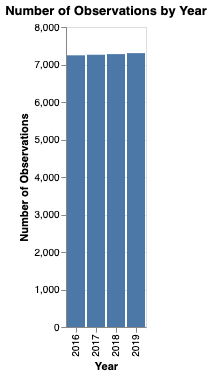
\includegraphics[width=2.08333in,height=\textheight,keepaspectratio]{s1p1.png}
4. a.

\begin{Shaded}
\begin{Highlighting}[]
\NormalTok{unique\_hospitals\_by\_year }\OperatorTok{=}\NormalTok{ all\_years\_data.groupby(}\StringTok{\textquotesingle{}YEAR\textquotesingle{}}\NormalTok{)[}\StringTok{\textquotesingle{}PRVDR\_NUM\textquotesingle{}}\NormalTok{].nunique().reset\_index(name}\OperatorTok{=}\StringTok{\textquotesingle{}unique\_count\textquotesingle{}}\NormalTok{)}

\NormalTok{unique\_hospital\_chart }\OperatorTok{=}\NormalTok{ alt.Chart(unique\_hospitals\_by\_year).mark\_bar().encode(}
\NormalTok{    x}\OperatorTok{=}\NormalTok{alt.X(}\StringTok{\textquotesingle{}YEAR:O\textquotesingle{}}\NormalTok{, title}\OperatorTok{=}\StringTok{\textquotesingle{}Year\textquotesingle{}}\NormalTok{),}
\NormalTok{    y}\OperatorTok{=}\NormalTok{alt.Y(}\StringTok{\textquotesingle{}unique\_count:Q\textquotesingle{}}\NormalTok{, title}\OperatorTok{=}\StringTok{\textquotesingle{}Number of Unique Hospitals\textquotesingle{}}\NormalTok{) }
\NormalTok{).properties(}
\NormalTok{    title}\OperatorTok{=}\StringTok{\textquotesingle{}Number of Unique Hospitals by Year\textquotesingle{}}
\NormalTok{)}
\NormalTok{unique\_hospital\_chart.display()}
\end{Highlighting}
\end{Shaded}

\begin{verbatim}
alt.Chart(...)
\end{verbatim}

\begin{figure}[H]

{\centering 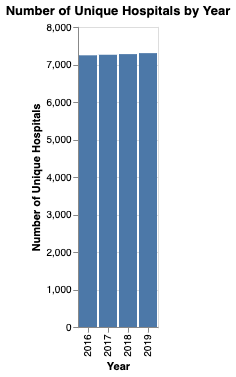
\includegraphics[width=2.08333in,height=\textheight,keepaspectratio]{s1p2.png}

}

\caption{unique hospitals}

\end{figure}%

\begin{enumerate}
\def\labelenumi{\alph{enumi}.}
\setcounter{enumi}{1}
\tightlist
\item
  The number of unique hospitals and total observations charts are
  identical, which means that each hospital has only one record in the
  dataset for each year. The dataset is structured as a snapshot of
  unique hospitals, with no intra-year variations or multiple records
  per hospital within each year.
\end{enumerate}

\subsection{Identify hospital closures in POS file (15 pts)
(*)}\label{identify-hospital-closures-in-pos-file-15-pts}

\begin{Shaded}
\begin{Highlighting}[]
\NormalTok{unique\_termination\_codes }\OperatorTok{=}\NormalTok{ all\_years\_data[}\StringTok{\textquotesingle{}PGM\_TRMNTN\_CD\textquotesingle{}}\NormalTok{].unique()}
\BuiltInTok{print}\NormalTok{(unique\_termination\_codes)}
\end{Highlighting}
\end{Shaded}

\begin{verbatim}
[0 1 7 4 6 5 3 2]
\end{verbatim}

\begin{enumerate}
\def\labelenumi{\arabic{enumi}.}
\tightlist
\item
\end{enumerate}

\begin{Shaded}
\begin{Highlighting}[]
\NormalTok{all\_years\_data[}\StringTok{\textquotesingle{}PGM\_TRMNTN\_CD\textquotesingle{}}\NormalTok{] }\OperatorTok{=}\NormalTok{ all\_years\_data[}\StringTok{\textquotesingle{}PGM\_TRMNTN\_CD\textquotesingle{}}\NormalTok{].astype(}\BuiltInTok{str}\NormalTok{)}
\NormalTok{all\_years\_data[}\StringTok{\textquotesingle{}PGM\_TRMNTN\_CD\textquotesingle{}}\NormalTok{] }\OperatorTok{=}\NormalTok{ all\_years\_data[}\StringTok{\textquotesingle{}PGM\_TRMNTN\_CD\textquotesingle{}}\NormalTok{].fillna(}\StringTok{\textquotesingle{}1\textquotesingle{}}\NormalTok{)}
\BuiltInTok{print}\NormalTok{(}\StringTok{"Check for missing values in PGM\_TRMNTN\_CD column after filling:"}\NormalTok{)}
\BuiltInTok{print}\NormalTok{(all\_years\_data[}\StringTok{\textquotesingle{}PGM\_TRMNTN\_CD\textquotesingle{}}\NormalTok{].isnull().}\BuiltInTok{sum}\NormalTok{()) }
\NormalTok{suspected\_closures }\OperatorTok{=}\NormalTok{ []}
\NormalTok{active\_2016 }\OperatorTok{=}\NormalTok{ all\_years\_data[(all\_years\_data[}\StringTok{\textquotesingle{}YEAR\textquotesingle{}}\NormalTok{] }\OperatorTok{==} \DecValTok{2016}\NormalTok{) }\OperatorTok{\&}\NormalTok{ (all\_years\_data[}\StringTok{\textquotesingle{}PGM\_TRMNTN\_CD\textquotesingle{}}\NormalTok{] }\OperatorTok{==} \StringTok{\textquotesingle{}0\textquotesingle{}}\NormalTok{)]}

\ControlFlowTok{for}\NormalTok{ \_, hospital }\KeywordTok{in}\NormalTok{ active\_2016.iterrows():}
\NormalTok{    facility\_name }\OperatorTok{=}\NormalTok{ hospital[}\StringTok{\textquotesingle{}FAC\_NAME\textquotesingle{}}\NormalTok{]}
\NormalTok{    zip\_code }\OperatorTok{=}\NormalTok{ hospital[}\StringTok{\textquotesingle{}ZIP\_CD\textquotesingle{}}\NormalTok{]}
    
\NormalTok{    closed\_2019 }\OperatorTok{=}\NormalTok{ all\_years\_data[}
\NormalTok{        (all\_years\_data[}\StringTok{\textquotesingle{}FAC\_NAME\textquotesingle{}}\NormalTok{] }\OperatorTok{==}\NormalTok{ facility\_name) }\OperatorTok{\&}
\NormalTok{        (all\_years\_data[}\StringTok{\textquotesingle{}ZIP\_CD\textquotesingle{}}\NormalTok{] }\OperatorTok{==}\NormalTok{ zip\_code) }\OperatorTok{\&}
\NormalTok{        (all\_years\_data[}\StringTok{\textquotesingle{}YEAR\textquotesingle{}}\NormalTok{] }\OperatorTok{==} \DecValTok{2019}\NormalTok{) }\OperatorTok{\&}
\NormalTok{        (all\_years\_data[}\StringTok{\textquotesingle{}PGM\_TRMNTN\_CD\textquotesingle{}}\NormalTok{].isin([}\StringTok{\textquotesingle{}1\textquotesingle{}}\NormalTok{, }\StringTok{\textquotesingle{}2\textquotesingle{}}\NormalTok{, }\StringTok{\textquotesingle{}3\textquotesingle{}}\NormalTok{, }\StringTok{\textquotesingle{}4\textquotesingle{}}\NormalTok{]))}
\NormalTok{    ]}
    
\NormalTok{    termination\_code\_2018 }\OperatorTok{=}\NormalTok{ all\_years\_data[}
\NormalTok{        (all\_years\_data[}\StringTok{\textquotesingle{}FAC\_NAME\textquotesingle{}}\NormalTok{] }\OperatorTok{==}\NormalTok{ facility\_name) }\OperatorTok{\&}
\NormalTok{        (all\_years\_data[}\StringTok{\textquotesingle{}ZIP\_CD\textquotesingle{}}\NormalTok{] }\OperatorTok{==}\NormalTok{ zip\_code) }\OperatorTok{\&}
\NormalTok{        (all\_years\_data[}\StringTok{\textquotesingle{}YEAR\textquotesingle{}}\NormalTok{] }\OperatorTok{==} \DecValTok{2018}\NormalTok{)}
\NormalTok{    ][}\StringTok{\textquotesingle{}PGM\_TRMNTN\_CD\textquotesingle{}}\NormalTok{].iloc[}\DecValTok{0}\NormalTok{] }\ControlFlowTok{if} \KeywordTok{not}\NormalTok{ all\_years\_data[}
\NormalTok{        (all\_years\_data[}\StringTok{\textquotesingle{}FAC\_NAME\textquotesingle{}}\NormalTok{] }\OperatorTok{==}\NormalTok{ facility\_name) }\OperatorTok{\&}
\NormalTok{        (all\_years\_data[}\StringTok{\textquotesingle{}ZIP\_CD\textquotesingle{}}\NormalTok{] }\OperatorTok{==}\NormalTok{ zip\_code) }\OperatorTok{\&}
\NormalTok{        (all\_years\_data[}\StringTok{\textquotesingle{}YEAR\textquotesingle{}}\NormalTok{] }\OperatorTok{==} \DecValTok{2018}\NormalTok{)}
\NormalTok{    ].empty }\ControlFlowTok{else} \VariableTok{None}

\NormalTok{    termination\_code\_2017 }\OperatorTok{=}\NormalTok{ all\_years\_data[}
\NormalTok{        (all\_years\_data[}\StringTok{\textquotesingle{}FAC\_NAME\textquotesingle{}}\NormalTok{] }\OperatorTok{==}\NormalTok{ facility\_name) }\OperatorTok{\&}
\NormalTok{        (all\_years\_data[}\StringTok{\textquotesingle{}ZIP\_CD\textquotesingle{}}\NormalTok{] }\OperatorTok{==}\NormalTok{ zip\_code) }\OperatorTok{\&}
\NormalTok{        (all\_years\_data[}\StringTok{\textquotesingle{}YEAR\textquotesingle{}}\NormalTok{] }\OperatorTok{==} \DecValTok{2017}\NormalTok{)}
\NormalTok{    ][}\StringTok{\textquotesingle{}PGM\_TRMNTN\_CD\textquotesingle{}}\NormalTok{].iloc[}\DecValTok{0}\NormalTok{] }\ControlFlowTok{if} \KeywordTok{not}\NormalTok{ all\_years\_data[}
\NormalTok{        (all\_years\_data[}\StringTok{\textquotesingle{}FAC\_NAME\textquotesingle{}}\NormalTok{] }\OperatorTok{==}\NormalTok{ facility\_name) }\OperatorTok{\&}
\NormalTok{        (all\_years\_data[}\StringTok{\textquotesingle{}ZIP\_CD\textquotesingle{}}\NormalTok{] }\OperatorTok{==}\NormalTok{ zip\_code) }\OperatorTok{\&}
\NormalTok{        (all\_years\_data[}\StringTok{\textquotesingle{}YEAR\textquotesingle{}}\NormalTok{] }\OperatorTok{==} \DecValTok{2017}\NormalTok{)}
\NormalTok{    ].empty }\ControlFlowTok{else} \VariableTok{None}
    
    \ControlFlowTok{if} \KeywordTok{not}\NormalTok{ closed\_2019.empty:}
\NormalTok{        suspected\_closures.append(\{}
            \StringTok{\textquotesingle{}FAC\_NAME\textquotesingle{}}\NormalTok{: facility\_name,}
            \StringTok{\textquotesingle{}ZIP\_CD\textquotesingle{}}\NormalTok{: zip\_code,}
            \StringTok{\textquotesingle{}year\_of\_closure\textquotesingle{}}\NormalTok{: }\DecValTok{2019}\NormalTok{,}
            \StringTok{\textquotesingle{}PGM\_TRMNTN\_CD\_2018\textquotesingle{}}\NormalTok{: termination\_code\_2018,}
            \StringTok{\textquotesingle{}PGM\_TRMNTN\_CD\_2017\textquotesingle{}}\NormalTok{: termination\_code\_2017}
\NormalTok{        \})}

\NormalTok{suspected\_closures\_df }\OperatorTok{=}\NormalTok{ pd.DataFrame(suspected\_closures).drop\_duplicates(subset}\OperatorTok{=}\NormalTok{[}\StringTok{\textquotesingle{}FAC\_NAME\textquotesingle{}}\NormalTok{, }\StringTok{\textquotesingle{}ZIP\_CD\textquotesingle{}}\NormalTok{])}

\NormalTok{num\_unique\_suspected\_closures }\OperatorTok{=} \BuiltInTok{len}\NormalTok{(suspected\_closures\_df)}
\BuiltInTok{print}\NormalTok{(}\SpecialStringTok{f"Number of unique hospitals suspected to have closed by 2019: }\SpecialCharTok{\{}\NormalTok{num\_unique\_suspected\_closures}\SpecialCharTok{\}}\SpecialStringTok{"}\NormalTok{)}
\end{Highlighting}
\end{Shaded}

\begin{verbatim}
Check for missing values in PGM_TRMNTN_CD column after filling:
0
Number of unique hospitals suspected to have closed by 2019: 145
\end{verbatim}

\begin{enumerate}
\def\labelenumi{\arabic{enumi}.}
\setcounter{enumi}{1}
\tightlist
\item
\end{enumerate}

\begin{Shaded}
\begin{Highlighting}[]
\BuiltInTok{print}\NormalTok{(suspected\_closures\_df.head(}\DecValTok{3}\NormalTok{))}
\end{Highlighting}
\end{Shaded}

\begin{verbatim}
                   FAC_NAME   ZIP_CD  year_of_closure PGM_TRMNTN_CD_2018  \
0  GEORGIANA MEDICAL CENTER  36033.0             2019                  0   
1          RMC JACKSONVILLE  36265.0             2019                  1   
2             UAB HIGHLANDS  35205.0             2019                  1   

  PGM_TRMNTN_CD_2017  
0                  0  
1                  0  
2                  1  
\end{verbatim}

\begin{enumerate}
\def\labelenumi{\arabic{enumi}.}
\setcounter{enumi}{2}
\tightlist
\item
  \begin{enumerate}
  \def\labelenumii{\alph{enumii}.}
  \tightlist
  \item
  \end{enumerate}
\end{enumerate}

\begin{Shaded}
\begin{Highlighting}[]
\NormalTok{properly\_closed\_hospitals }\OperatorTok{=}\NormalTok{ []}
\NormalTok{merge\_hospitals }\OperatorTok{=}\NormalTok{ []}

\ControlFlowTok{for}\NormalTok{ \_, hospital }\KeywordTok{in}\NormalTok{ suspected\_closures\_df.iterrows():}
\NormalTok{    facility\_name }\OperatorTok{=}\NormalTok{ hospital[}\StringTok{\textquotesingle{}FAC\_NAME\textquotesingle{}}\NormalTok{]}
\NormalTok{    zip\_code }\OperatorTok{=}\NormalTok{ hospital[}\StringTok{\textquotesingle{}ZIP\_CD\textquotesingle{}}\NormalTok{]}
\NormalTok{    termination\_code\_2018 }\OperatorTok{=}\NormalTok{ hospital[}\StringTok{\textquotesingle{}PGM\_TRMNTN\_CD\_2018\textquotesingle{}}\NormalTok{]}
\NormalTok{    termination\_code\_2017 }\OperatorTok{=}\NormalTok{ hospital[}\StringTok{\textquotesingle{}PGM\_TRMNTN\_CD\_2017\textquotesingle{}}\NormalTok{]}
    
    \ControlFlowTok{if}\NormalTok{ termination\_code\_2018 }\OperatorTok{!=} \StringTok{\textquotesingle{}0\textquotesingle{}}\NormalTok{:}
\NormalTok{        properly\_closed\_hospitals.append(\{}
            \StringTok{\textquotesingle{}FAC\_NAME\textquotesingle{}}\NormalTok{: facility\_name,}
            \StringTok{\textquotesingle{}ZIP\_CD\textquotesingle{}}\NormalTok{: zip\_code,}
            \StringTok{\textquotesingle{}PGM\_TRMNTN\_CD\_2018\textquotesingle{}}\NormalTok{: termination\_code\_2018,}
            \StringTok{\textquotesingle{}PGM\_TRMNTN\_CD\_2017\textquotesingle{}}\NormalTok{: termination\_code\_2017}
\NormalTok{        \})}
    \ControlFlowTok{else}\NormalTok{:}
        \ControlFlowTok{if}\NormalTok{ termination\_code\_2017 }\OperatorTok{==} \StringTok{\textquotesingle{}0\textquotesingle{}}\NormalTok{:}
\NormalTok{            properly\_closed\_hospitals.append(\{}
                \StringTok{\textquotesingle{}FAC\_NAME\textquotesingle{}}\NormalTok{: facility\_name,}
                \StringTok{\textquotesingle{}ZIP\_CD\textquotesingle{}}\NormalTok{: zip\_code,}
                \StringTok{\textquotesingle{}PGM\_TRMNTN\_CD\_2018\textquotesingle{}}\NormalTok{: termination\_code\_2018,}
                \StringTok{\textquotesingle{}PGM\_TRMNTN\_CD\_2017\textquotesingle{}}\NormalTok{: termination\_code\_2017}
\NormalTok{            \})}
        \ControlFlowTok{else}\NormalTok{:}
\NormalTok{            merge\_hospitals.append(\{}
                \StringTok{\textquotesingle{}FAC\_NAME\textquotesingle{}}\NormalTok{: facility\_name,}
                \StringTok{\textquotesingle{}ZIP\_CD\textquotesingle{}}\NormalTok{: zip\_code,}
                \StringTok{\textquotesingle{}PGM\_TRMNTN\_CD\_2018\textquotesingle{}}\NormalTok{: termination\_code\_2018,}
                \StringTok{\textquotesingle{}PGM\_TRMNTN\_CD\_2017\textquotesingle{}}\NormalTok{: termination\_code\_2017}
\NormalTok{            \})}
\NormalTok{properly\_closed\_hospitals\_df }\OperatorTok{=}\NormalTok{ pd.DataFrame(properly\_closed\_hospitals)}
\NormalTok{merge\_hospitals\_df }\OperatorTok{=}\NormalTok{ pd.DataFrame(merge\_hospitals)}

\BuiltInTok{print}\NormalTok{(}\StringTok{"Properly closed hospitals:"}\NormalTok{)}
\BuiltInTok{print}\NormalTok{(properly\_closed\_hospitals\_df.head(}\DecValTok{3}\NormalTok{))}

\BuiltInTok{print}\NormalTok{(}\StringTok{"}\CharTok{\textbackslash{}n}\StringTok{Hospitals suspected of merger:"}\NormalTok{)}
\BuiltInTok{print}\NormalTok{(merge\_hospitals\_df.head(}\DecValTok{3}\NormalTok{))}

\NormalTok{num\_properly\_closed }\OperatorTok{=}\NormalTok{ properly\_closed\_hospitals\_df.shape[}\DecValTok{0}\NormalTok{]}
\BuiltInTok{print}\NormalTok{(}\SpecialStringTok{f"Number of properly closed hospitals: }\SpecialCharTok{\{}\NormalTok{num\_properly\_closed}\SpecialCharTok{\}}\SpecialStringTok{"}\NormalTok{)}

\NormalTok{num\_suspected\_mergers }\OperatorTok{=}\NormalTok{ merge\_hospitals\_df.shape[}\DecValTok{0}\NormalTok{]}
\BuiltInTok{print}\NormalTok{(}\SpecialStringTok{f"Number of suspected mergers: }\SpecialCharTok{\{}\NormalTok{num\_suspected\_mergers}\SpecialCharTok{\}}\SpecialStringTok{"}\NormalTok{)}
\end{Highlighting}
\end{Shaded}

\begin{verbatim}
Properly closed hospitals:
                   FAC_NAME   ZIP_CD PGM_TRMNTN_CD_2018 PGM_TRMNTN_CD_2017
0  GEORGIANA MEDICAL CENTER  36033.0                  0                  0
1          RMC JACKSONVILLE  36265.0                  1                  0
2             UAB HIGHLANDS  35205.0                  1                  1

Hospitals suspected of merger:
Empty DataFrame
Columns: []
Index: []
Number of properly closed hospitals: 145
Number of suspected mergers: 0
\end{verbatim}

\begin{Shaded}
\begin{Highlighting}[]
\NormalTok{properly\_closed\_hospitals }\OperatorTok{=}\NormalTok{ []}
\NormalTok{merge\_hospitals }\OperatorTok{=}\NormalTok{ []}

\ControlFlowTok{for}\NormalTok{ \_, hospital }\KeywordTok{in}\NormalTok{ suspected\_closures\_df.iterrows():}
\NormalTok{    facility\_name }\OperatorTok{=}\NormalTok{ hospital[}\StringTok{\textquotesingle{}FAC\_NAME\textquotesingle{}}\NormalTok{]}
\NormalTok{    zip\_code }\OperatorTok{=}\NormalTok{ hospital[}\StringTok{\textquotesingle{}ZIP\_CD\textquotesingle{}}\NormalTok{]}
    
\NormalTok{    hospital\_data }\OperatorTok{=}\NormalTok{ all\_years\_data[}
\NormalTok{        (all\_years\_data[}\StringTok{\textquotesingle{}FAC\_NAME\textquotesingle{}}\NormalTok{] }\OperatorTok{==}\NormalTok{ facility\_name) }\OperatorTok{\&} 
\NormalTok{        (all\_years\_data[}\StringTok{\textquotesingle{}ZIP\_CD\textquotesingle{}}\NormalTok{] }\OperatorTok{==}\NormalTok{ zip\_code) }\OperatorTok{\&}
\NormalTok{        (all\_years\_data[}\StringTok{\textquotesingle{}YEAR\textquotesingle{}}\NormalTok{].isin([}\DecValTok{2017}\NormalTok{, }\DecValTok{2018}\NormalTok{]))}
\NormalTok{    ]}

\NormalTok{    termination\_2018 }\OperatorTok{=}\NormalTok{ hospital\_data[hospital\_data[}\StringTok{\textquotesingle{}YEAR\textquotesingle{}}\NormalTok{] }\OperatorTok{==} \DecValTok{2018}\NormalTok{][}\StringTok{\textquotesingle{}PGM\_TRMNTN\_CD\textquotesingle{}}\NormalTok{].iloc[}\DecValTok{0}\NormalTok{] }\ControlFlowTok{if} \KeywordTok{not}\NormalTok{ hospital\_data[hospital\_data[}\StringTok{\textquotesingle{}YEAR\textquotesingle{}}\NormalTok{] }\OperatorTok{==} \DecValTok{2018}\NormalTok{].empty }\ControlFlowTok{else} \StringTok{\textquotesingle{}1\textquotesingle{}}
\NormalTok{    termination\_2017 }\OperatorTok{=}\NormalTok{ hospital\_data[hospital\_data[}\StringTok{\textquotesingle{}YEAR\textquotesingle{}}\NormalTok{] }\OperatorTok{==} \DecValTok{2017}\NormalTok{][}\StringTok{\textquotesingle{}PGM\_TRMNTN\_CD\textquotesingle{}}\NormalTok{].iloc[}\DecValTok{0}\NormalTok{] }\ControlFlowTok{if} \KeywordTok{not}\NormalTok{ hospital\_data[hospital\_data[}\StringTok{\textquotesingle{}YEAR\textquotesingle{}}\NormalTok{] }\OperatorTok{==} \DecValTok{2017}\NormalTok{].empty }\ControlFlowTok{else} \StringTok{\textquotesingle{}1\textquotesingle{}}

    \ControlFlowTok{if}\NormalTok{ termination\_2018 }\OperatorTok{!=} \StringTok{\textquotesingle{}0\textquotesingle{}}\NormalTok{:}
\NormalTok{        properly\_closed\_hospitals.append(\{}
            \StringTok{\textquotesingle{}FAC\_NAME\textquotesingle{}}\NormalTok{: facility\_name,}
            \StringTok{\textquotesingle{}ZIP\_CD\textquotesingle{}}\NormalTok{: zip\_code,}
            \StringTok{\textquotesingle{}PGM\_TRMNTN\_CD\_2017\textquotesingle{}}\NormalTok{: termination\_2017,}
            \StringTok{\textquotesingle{}PGM\_TRMNTN\_CD\_2018\textquotesingle{}}\NormalTok{: termination\_2018}
\NormalTok{        \})}
    \ControlFlowTok{elif}\NormalTok{ termination\_2018 }\OperatorTok{==} \StringTok{\textquotesingle{}0\textquotesingle{}}\NormalTok{:}
        \ControlFlowTok{if}\NormalTok{ termination\_2017 }\OperatorTok{==} \StringTok{\textquotesingle{}0\textquotesingle{}}\NormalTok{:}
\NormalTok{            properly\_closed\_hospitals.append(\{}
                \StringTok{\textquotesingle{}FAC\_NAME\textquotesingle{}}\NormalTok{: facility\_name,}
                \StringTok{\textquotesingle{}ZIP\_CD\textquotesingle{}}\NormalTok{: zip\_code,}
                \StringTok{\textquotesingle{}PGM\_TRMNTN\_CD\_2017\textquotesingle{}}\NormalTok{: termination\_2017,}
                \StringTok{\textquotesingle{}PGM\_TRMNTN\_CD\_2018\textquotesingle{}}\NormalTok{: termination\_2018}
\NormalTok{            \})}
        \ControlFlowTok{else}\NormalTok{:}
            \CommentTok{\# Otherwise, add to suspected mergers}
\NormalTok{            merge\_hospitals.append(\{}
                \StringTok{\textquotesingle{}FAC\_NAME\textquotesingle{}}\NormalTok{: facility\_name,}
                \StringTok{\textquotesingle{}ZIP\_CD\textquotesingle{}}\NormalTok{: zip\_code,}
                \StringTok{\textquotesingle{}PGM\_TRMNTN\_CD\_2017\textquotesingle{}}\NormalTok{: termination\_2017,}
                \StringTok{\textquotesingle{}PGM\_TRMNTN\_CD\_2018\textquotesingle{}}\NormalTok{: termination\_2018}
\NormalTok{            \})}

\CommentTok{\# Convert results to DataFrames for inspection}
\NormalTok{properly\_closed\_hospitals\_df }\OperatorTok{=}\NormalTok{ pd.DataFrame(properly\_closed\_hospitals)}
\NormalTok{merge\_hospitals\_df }\OperatorTok{=}\NormalTok{ pd.DataFrame(merge\_hospitals)}
\CommentTok{\# Number of properly closed hospitals}
\NormalTok{num\_properly\_closed }\OperatorTok{=}\NormalTok{ properly\_closed\_hospitals\_df.shape[}\DecValTok{0}\NormalTok{]}
\BuiltInTok{print}\NormalTok{(}\SpecialStringTok{f"Number of properly closed hospitals: }\SpecialCharTok{\{}\NormalTok{num\_properly\_closed}\SpecialCharTok{\}}\SpecialStringTok{"}\NormalTok{)}

\CommentTok{\# Number of suspected mergers}
\NormalTok{num\_suspected\_mergers }\OperatorTok{=}\NormalTok{ merge\_hospitals\_df.shape[}\DecValTok{0}\NormalTok{]}
\BuiltInTok{print}\NormalTok{(}\SpecialStringTok{f"Number of suspected mergers: }\SpecialCharTok{\{}\NormalTok{num\_suspected\_mergers}\SpecialCharTok{\}}\SpecialStringTok{"}\NormalTok{)}
\end{Highlighting}
\end{Shaded}

\begin{verbatim}
Number of properly closed hospitals: 145
Number of suspected mergers: 0
\end{verbatim}

There are no potential merged hospitals! a. there are no merged
hospitals! b.

\begin{verbatim}
# Sort the properly closed hospitals by FAC_NAME and display the first 10 rows
\end{verbatim}

sorted\_properly\_closed\_hospitals =
properly\_closed\_hospitals\_df.sort\_values(by=`FAC\_NAME').head(3)

\section{Display the sorted list}\label{display-the-sorted-list}

print(``First 10 corrected hospital closures sorted by name:'')
print(sorted\_properly\_closed\_hospitals.head(3))

\begin{verbatim}


## Download Census zip code shapefile (10 pt) 

1. 
    a. There are five types of file types here. 
**.shp (shape file)**: file contains the geometric shapes. It stores the spatial coordinates and shapes of objects like points, lines or polygons. 
**.shx (shape index format)**: file is an index of the geometry in the .shp file, and provides quick access to the geometric shapes. 
**.dbf (attribute format)**: file contains attribute data in tabular format, with each row corresponding to a feature and each column containing attributes associated with that feature. 
**.prj (projection format)**: file contains information about the coordinate sysetm and projection, and defines how shapes are mapped onto Earth's surface. 
**.xml (metadata format)**: file contains metadata, contains descriptive information about dataset such as source, creation date, projection dates. 

    b. 
| File Extension | Size (MB)  |
|----------------|------------|
| .shp           | 837.5      |
| .dbf           | 6.4        |
| .prj           | 0.000165   |
| .shx           | 0.000265   |
| .xml           | 0.016      |

2. 

```{python}
import geopandas as gpd
\end{verbatim}

\begin{Shaded}
\begin{Highlighting}[]
\NormalTok{shapefile\_path = \textquotesingle{}/Users/samarnegahdar/Desktop/untitled folder/problem{-}set{-}4{-}summer{-}jenny/shapefiles/gz\_2010\_us\_860\_00\_500k.shp\textquotesingle{}}

\NormalTok{try:}
\NormalTok{    zip\_shapes = gpd.read\_file(shapefile\_path)}
\NormalTok{    print("Shapefile loaded successfully with SHX restoration.")}
\NormalTok{except Exception as e:}
\NormalTok{    print("Error loading shapefile:", e)}
\end{Highlighting}
\end{Shaded}

\begin{Shaded}
\begin{Highlighting}[]
\NormalTok{\#filtering for texas zip codes}
\NormalTok{texas\_zip\_shapes = zip\_shapes[zip\_shapes[\textquotesingle{}ZCTA5\textquotesingle{}].astype(str).str.startswith((\textquotesingle{}75\textquotesingle{}, \textquotesingle{}76\textquotesingle{}, \textquotesingle{}77\textquotesingle{}, \textquotesingle{}78\textquotesingle{}, \textquotesingle{}79\textquotesingle{})) | (zip\_shapes[\textquotesingle{}ZCTA5\textquotesingle{}] == \textquotesingle{}733\textquotesingle{})]}

\NormalTok{print(texas\_zip\_shapes.head(3))}
\NormalTok{print("Number of Texas ZIP codes:", texas\_zip\_shapes.shape[0])}
\end{Highlighting}
\end{Shaded}

\begin{Shaded}
\begin{Highlighting}[]
\NormalTok{\#pos2016 }
\NormalTok{pos2016[\textquotesingle{}ZIP\_CD\textquotesingle{}] = pos2016[\textquotesingle{}ZIP\_CD\textquotesingle{}].astype(str)}

\NormalTok{texas\_hospitals\_2016 = pos2016[pos2016[\textquotesingle{}ZIP\_CD\textquotesingle{}].str.startswith((\textquotesingle{}75\textquotesingle{}, \textquotesingle{}76\textquotesingle{}, \textquotesingle{}77\textquotesingle{}, \textquotesingle{}78\textquotesingle{}, \textquotesingle{}79\textquotesingle{})) | (pos2016[\textquotesingle{}ZIP\_CD\textquotesingle{}] == \textquotesingle{}733\textquotesingle{})]}

\NormalTok{print(texas\_hospitals\_2016.head(3))}
\NormalTok{print("Number of Texas hospital records in 2016:", texas\_hospitals\_2016.shape[0])}

\NormalTok{hospitals\_per\_zip = texas\_hospitals\_2016.groupby(\textquotesingle{}ZIP\_CD\textquotesingle{}).size().reset\_index(name=\textquotesingle{}hospital\_count\textquotesingle{})}
\end{Highlighting}
\end{Shaded}

\begin{Shaded}
\begin{Highlighting}[]
\NormalTok{texas\_zip\_shapes[\textquotesingle{}ZCTA5\textquotesingle{}] = texas\_zip\_shapes[\textquotesingle{}ZCTA5\textquotesingle{}].astype(str)}
\NormalTok{hospitals\_per\_zip[\textquotesingle{}ZIP\_CD\textquotesingle{}] = hospitals\_per\_zip[\textquotesingle{}ZIP\_CD\textquotesingle{}].astype(float).astype(int).astype(str).str.zfill(5)}
\NormalTok{print("Formatted ZIP codes in hospitals\_per\_zip:", hospitals\_per\_zip[\textquotesingle{}ZIP\_CD\textquotesingle{}].unique()[:10])}
\NormalTok{hospitals\_per\_zip = hospitals\_per\_zip[[\textquotesingle{}ZIP\_CD\textquotesingle{}, \textquotesingle{}hospital\_count\textquotesingle{}]]}
\NormalTok{hospitals\_per\_zip = hospitals\_per\_zip.rename(columns=\{\textquotesingle{}ZIP\_CD\textquotesingle{}: \textquotesingle{}ZIP\_CD\_hp\textquotesingle{}, \textquotesingle{}hospital\_count\textquotesingle{}: \textquotesingle{}hospital\_count\_hp\textquotesingle{}\})}
\NormalTok{texas\_zip\_shapes = texas\_zip\_shapes.merge(hospitals\_per\_zip, left\_on=\textquotesingle{}ZCTA5\textquotesingle{}, right\_on=\textquotesingle{}ZIP\_CD\_hp\textquotesingle{}, how=\textquotesingle{}left\textquotesingle{})}
\NormalTok{texas\_zip\_shapes[\textquotesingle{}hospital\_count\_hp\textquotesingle{}] = texas\_zip\_shapes[\textquotesingle{}hospital\_count\_hp\textquotesingle{}].fillna(0)}
\NormalTok{print("Number of ZIP codes with hospital\_count as 0:", (texas\_zip\_shapes[\textquotesingle{}hospital\_count\_hp\textquotesingle{}] == 0).sum())}
\NormalTok{print("Total ZIP codes in Texas:", texas\_zip\_shapes.shape[0])}
\NormalTok{print(texas\_zip\_shapes[[\textquotesingle{}ZCTA5\textquotesingle{}, \textquotesingle{}hospital\_count\_hp\textquotesingle{}]].head(3))}
\end{Highlighting}
\end{Shaded}

\begin{Shaded}
\begin{Highlighting}[]
\NormalTok{import matplotlib.pyplot as plt}

\NormalTok{fig, ax = plt.subplots(1, 1, figsize=(12, 10))}
\NormalTok{texas\_zip\_shapes.plot(column=\textquotesingle{}hospital\_count\_hp\textquotesingle{}, cmap=\textquotesingle{}OrRd\textquotesingle{}, linewidth=0.8, ax=ax, edgecolor=\textquotesingle{}0.8\textquotesingle{}, legend=True)}
\NormalTok{ax.set\_title("Number of Hospitals per ZIP Code in Texas (2016)")}
\NormalTok{ax.set\_axis\_off()}
\NormalTok{plt.show()}
\end{Highlighting}
\end{Shaded}

\begin{figure}[H]

{\centering 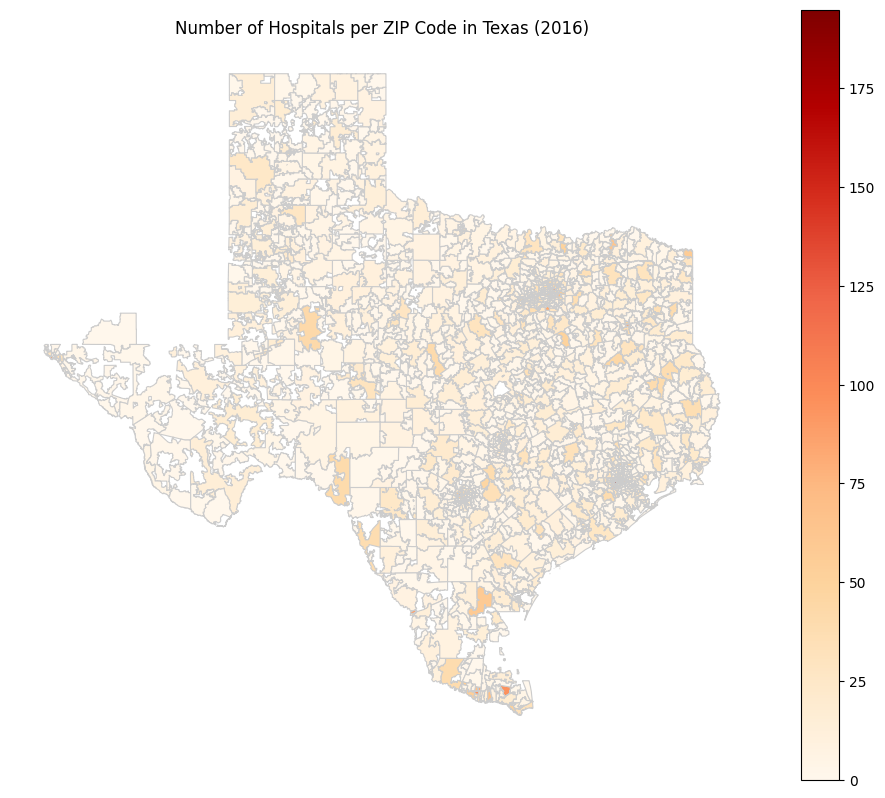
\includegraphics[width=6.25in,height=\textheight,keepaspectratio]{s3q1.png}

}

\caption{hospitals/zipcode}

\end{figure}%

\subsection{Calculate zip code's distance to the nearest hospital (20
pts)
(*)}\label{calculate-zip-codes-distance-to-the-nearest-hospital-20-pts}

\begin{enumerate}
\def\labelenumi{\arabic{enumi}.}
\tightlist
\item
\end{enumerate}

\begin{Shaded}
\begin{Highlighting}[]
\NormalTok{zip\_shapes[\textquotesingle{}centroids\textquotesingle{}]= zip\_shapes.geometry.centroid}
\NormalTok{all\_zip\_centroid= zip\_shapes.copy().set\_geometry(\textquotesingle{}centroids\textquotesingle{})}
\NormalTok{print(all\_zip\_centroid.shape.head(3))}
\NormalTok{print(all\_zip\_centroid.columns.head(3))}
\NormalTok{print(all\_zip\_centroid.head(3))}
\end{Highlighting}
\end{Shaded}

GEO\_ID: it is ta code to identify the grographic type: state, county,
zipcode

ZCTA5:it is 5 digit zip code tabulation area(approximation of postal
codes)

NAME: is the same as ZCTA5 only more user friendly.

LSDA: legal/statistical area description categorizing geo area type(
state, county,zipcode(in this case our description is zip code ZCTA5))

CENSUSAREA:The land area of the ZCTA in square miles as calculated by
the Census Bureau. It measures the physical size of each area, excluding
water bodies.

\begin{enumerate}
\def\labelenumi{\arabic{enumi}.}
\setcounter{enumi}{1}
\tightlist
\item
\end{enumerate}

\begin{Shaded}
\begin{Highlighting}[]
\NormalTok{from shapely.ops import unary\_union}

\NormalTok{zips\_texas\_centroids = all\_zip\_centroid[all\_zip\_centroid[\textquotesingle{}ZCTA5\textquotesingle{}].str.startswith((\textquotesingle{}75\textquotesingle{}, \textquotesingle{}76\textquotesingle{}, \textquotesingle{}77\textquotesingle{}, \textquotesingle{}78\textquotesingle{}, \textquotesingle{}79\textquotesingle{}))]}

\NormalTok{zips\_texas\_borderstates\_centroids = all\_zip\_centroid[all\_zip\_centroid[\textquotesingle{}ZCTA5\textquotesingle{}].str.startswith(}
\NormalTok{    (\textquotesingle{}75\textquotesingle{}, \textquotesingle{}76\textquotesingle{}, \textquotesingle{}77\textquotesingle{}, \textquotesingle{}78\textquotesingle{}, \textquotesingle{}79\textquotesingle{}, \textquotesingle{}70\textquotesingle{}, \textquotesingle{}71\textquotesingle{}, \textquotesingle{}72\textquotesingle{}, \textquotesingle{}73\textquotesingle{}, \textquotesingle{}74\textquotesingle{}, \textquotesingle{}80\textquotesingle{}, \textquotesingle{}81\textquotesingle{}, \textquotesingle{}88\textquotesingle{}, \textquotesingle{}87\textquotesingle{}, \textquotesingle{}86\textquotesingle{})}
\NormalTok{)]}

\NormalTok{num\_texas\_zips = zips\_texas\_centroids[\textquotesingle{}ZCTA5\textquotesingle{}].nunique()}
\NormalTok{num\_bordering\_zips = zips\_texas\_borderstates\_centroids[\textquotesingle{}ZCTA5\textquotesingle{}].nunique()}
\NormalTok{print(f"Number of unique Texas ZIP codes: \{num\_texas\_zips\}")}
\NormalTok{print(f"Number of unique ZIP codes in Texas and bordering states: \{num\_bordering\_zips\}")}
\NormalTok{def intersects\_texas(texas\_polygon, other\_polygon):}
\NormalTok{    return texas\_polygon.intersects(other\_polygon)}

\NormalTok{texas\_polygon = unary\_union(zips\_texas\_centroids.geometry)}

\NormalTok{zips\_texas\_borderstates\_centroids[\textquotesingle{}borders\_texas\textquotesingle{}] = zips\_texas\_borderstates\_centroids.geometry.apply(}
\NormalTok{    lambda geom: intersects\_texas(texas\_polygon, geom)}
\NormalTok{)}

\NormalTok{unique\_texas\_zips = zips\_texas\_centroids[\textquotesingle{}ZCTA5\textquotesingle{}].nunique()}
\NormalTok{unique\_bordering\_zips = zips\_texas\_borderstates\_centroids[zips\_texas\_borderstates\_centroids[\textquotesingle{}borders\_texas\textquotesingle{}]][\textquotesingle{}ZCTA5\textquotesingle{}].nunique()}

\NormalTok{print(f"Unique Texas ZIP codes: \{unique\_texas\_zips\}")}
\NormalTok{print(f"Unique ZIP codes in Texas and bordering states: \{unique\_bordering\_zips\}")}
\end{Highlighting}
\end{Shaded}

\begin{enumerate}
\def\labelenumi{\arabic{enumi}.}
\setcounter{enumi}{2}
\tightlist
\item
\end{enumerate}

\begin{Shaded}
\begin{Highlighting}[]
\NormalTok{texas\_hospitals\_2016 = pos2016[pos2016[\textquotesingle{}ZIP\_CD\textquotesingle{}].str.startswith((\textquotesingle{}75\textquotesingle{}, \textquotesingle{}76\textquotesingle{}, \textquotesingle{}77\textquotesingle{}, \textquotesingle{}78\textquotesingle{}, \textquotesingle{}79\textquotesingle{})) | (pos2016[\textquotesingle{}ZIP\_CD\textquotesingle{}] == \textquotesingle{}733\textquotesingle{})]}
\NormalTok{hospitals\_per\_zip = texas\_hospitals\_2016.groupby(\textquotesingle{}ZIP\_CD\textquotesingle{}).size().reset\_index(name=\textquotesingle{}hospital\_count\textquotesingle{})}
\NormalTok{hospitals\_per\_zip[\textquotesingle{}ZIP\_CD\textquotesingle{}] = hospitals\_per\_zip[\textquotesingle{}ZIP\_CD\textquotesingle{}].astype(str).str.zfill(5)}

\NormalTok{zips\_texas\_borderstates\_centroids[\textquotesingle{}ZCTA5\textquotesingle{}] = zips\_texas\_borderstates\_centroids[\textquotesingle{}ZCTA5\textquotesingle{}].astype(str).str.zfill(5)}

\NormalTok{print("Sample ZIP codes in hospitals\_per\_zip (should be string with zero{-}padding):")}
\NormalTok{print(hospitals\_per\_zip[\textquotesingle{}ZIP\_CD\textquotesingle{}].head(3))}

\NormalTok{print("Sample ZIP codes in zips\_texas\_borderstates\_centroids (should be string with zero{-}padding):")}
\NormalTok{print(zips\_texas\_borderstates\_centroids[\textquotesingle{}ZCTA5\textquotesingle{}].head(3))}

\NormalTok{zips\_withhospital\_centroids = zips\_texas\_borderstates\_centroids.merge(}
\NormalTok{    hospitals\_per\_zip,}
\NormalTok{    left\_on=\textquotesingle{}ZCTA5\textquotesingle{},}
\NormalTok{    right\_on=\textquotesingle{}ZIP\_CD\textquotesingle{},}
\NormalTok{    how=\textquotesingle{}inner\textquotesingle{}}
\NormalTok{)}

\NormalTok{zips\_withhospital\_centroids = zips\_withhospital\_centroids[zips\_withhospital\_centroids[\textquotesingle{}hospital\_count\textquotesingle{}] \textgreater{} 0]}

\NormalTok{print("zips\_withhospital\_centroids with at least 1 hospital:")}
\NormalTok{print(zips\_withhospital\_centroids.head(3))}
\NormalTok{num\_unique\_zip\_codes = zips\_withhospital\_centroids[\textquotesingle{}ZCTA5\textquotesingle{}].nunique()}
\NormalTok{print(f"Number of unique ZIP codes with at least 1 hospital in 2016: \{num\_unique\_zip\_codes\}")}
\end{Highlighting}
\end{Shaded}

I inner merged on zip code but had osme problems because they did not
match (zip code in geo file had decimals and had to be converted)

\begin{enumerate}
\def\labelenumi{\arabic{enumi}.}
\setcounter{enumi}{3}
\tightlist
\item
  \begin{enumerate}
  \def\labelenumii{\alph{enumii}.}
  \tightlist
  \item
  \end{enumerate}
\end{enumerate}

\begin{Shaded}
\begin{Highlighting}[]
\NormalTok{import numpy as np}
\NormalTok{import time}
\NormalTok{start\_time\_T= time.time()}
\NormalTok{LAT\_TO\_MILES = 69.0  }
\NormalTok{LON\_TO\_MILES = 55.0 }

\NormalTok{def degree\_to\_miles\_distance(point1, point2):}
\NormalTok{    lat\_diff = (point1.y {-} point2.y) * LAT\_TO\_MILES}
\NormalTok{    lon\_diff = (point1.x {-} point2.x) * LON\_TO\_MILES}
\NormalTok{    return np.sqrt(lat\_diff**2 + lon\_diff**2)}

\NormalTok{def calculate\_nearest\_distance(point, centroids):}
\NormalTok{    if centroids.empty:}
\NormalTok{        return float(\textquotesingle{}inf\textquotesingle{})  \# Return infinity if there are no centroids}
\NormalTok{    return min(degree\_to\_miles\_distance(point, centroid) for centroid in centroids)}

\NormalTok{Q4a\_subset = zips\_texas\_centroids.head(3)}
\NormalTok{start\_time = time.time()}

\NormalTok{Q4a\_subset[\textquotesingle{}nearest\_hospital\_distance\textquotesingle{}] = Q4a\_subset[\textquotesingle{}centroids\textquotesingle{}].apply(}
\NormalTok{    lambda x: calculate\_nearest\_distance(x, zips\_withhospital\_centroids[\textquotesingle{}centroids\textquotesingle{}])}
\NormalTok{)}

\NormalTok{end\_time = time.time()}
\NormalTok{subset\_duration = end\_time {-} start\_time}
\NormalTok{total\_zips\_count = len(zips\_texas\_centroids)}
\NormalTok{estimated\_total\_duration = (subset\_duration / 10) * total\_zips\_count}

\NormalTok{print(f"Time taken for 10 ZIP codes: \{subset\_duration:.2f\} seconds")}
\NormalTok{print(f"Estimated time for entire dataset: \{estimated\_total\_duration / 60:.2f\} minutes")}
\end{Highlighting}
\end{Shaded}

It will take approximatelty 18 seconds to run the whole dataset! b. look
at part C where I calculated the actual distance. I have mentioned how
much it will take to run the whole thing there. it is 36 seconds! c. the
unit is degree, which is approximately 69 miles or 111 km. here is
convertion:

\begin{Shaded}
\begin{Highlighting}[]
\NormalTok{start\_time\_T= time.time()}

\NormalTok{zips\_texas\_centroids[\textquotesingle{}nearest\_hospital\_distance\_miles\textquotesingle{}] = zips\_texas\_centroids[\textquotesingle{}centroids\textquotesingle{}].apply(}
\NormalTok{    lambda centroid: min(}
\NormalTok{        degree\_to\_miles\_distance(centroid, hospital\_centroid) }
\NormalTok{        for hospital\_centroid in zips\_withhospital\_centroids[\textquotesingle{}centroids\textquotesingle{}]}
\NormalTok{    )}
\NormalTok{)}

\NormalTok{average\_distance\_miles = zips\_texas\_centroids[\textquotesingle{}nearest\_hospital\_distance\_miles\textquotesingle{}].mean()}
\NormalTok{end\_time\_T=time.time()}
\NormalTok{total\_time= end\_time\_T {-} start\_time\_T}
\NormalTok{print(f"The average distance to the nearest hospital in Texas (in miles) is: \{average\_distance\_miles:.2f\}", "miles")}
\NormalTok{print("the total time required to calculate the prompt above is", total\_time, "seconds")}
\end{Highlighting}
\end{Shaded}

\begin{enumerate}
\def\labelenumi{\arabic{enumi}.}
\setcounter{enumi}{4}
\tightlist
\item
\end{enumerate}

\begin{Shaded}
\begin{Highlighting}[]

\NormalTok{average\_distance = zips\_texas\_centroids[\textquotesingle{}nearest\_hospital\_distance\_miles\textquotesingle{}].mean()}
\NormalTok{print(f"Average distance to the nearest hospital for each ZIP code in Texas: \{average\_distance:.2f\} miles")}

\NormalTok{fig, ax = plt.subplots(1, 1, figsize=(12, 10))}
\NormalTok{zips\_texas\_centroids.plot(column=\textquotesingle{}nearest\_hospital\_distance\_miles\textquotesingle{}, cmap=\textquotesingle{}YlOrRd\textquotesingle{}, linewidth=0.8, ax=ax, edgecolor=\textquotesingle{}0.8\textquotesingle{}, legend=True)}
\NormalTok{ax.set\_title("Distance to the Nearest Hospital for Each ZIP Code in Texas (Miles)")}
\NormalTok{ax.set\_axis\_off()}
\NormalTok{plt.show()}
\end{Highlighting}
\end{Shaded}

\subsection{Effects of closures on access in Texas (15
pts)}\label{effects-of-closures-on-access-in-texas-15-pts}

\begin{enumerate}
\def\labelenumi{\arabic{enumi}.}
\tightlist
\item
  There are 20 hospitals that have had at least one closure between
  2016-2019.
\end{enumerate}

\begin{Shaded}
\begin{Highlighting}[]
\NormalTok{corrected\_closures\_df = pd.DataFrame(properly\_closed\_hospitals)}

\NormalTok{corrected\_closures\_df[\textquotesingle{}ZIP\_CD\textquotesingle{}] = corrected\_closures\_df[\textquotesingle{}ZIP\_CD\textquotesingle{}].astype(str)}
\NormalTok{texas\_closures = corrected\_closures\_df[corrected\_closures\_df[\textquotesingle{}ZIP\_CD\textquotesingle{}].str.startswith((\textquotesingle{}75\textquotesingle{}, \textquotesingle{}76\textquotesingle{}, \textquotesingle{}77\textquotesingle{}, \textquotesingle{}78\textquotesingle{}, \textquotesingle{}79\textquotesingle{}, \textquotesingle{}733\textquotesingle{}))]}
\NormalTok{closures\_by\_zip = texas\_closures.groupby(\textquotesingle{}ZIP\_CD\textquotesingle{}).size().reset\_index(name=\textquotesingle{}closure\_count\textquotesingle{})}

\NormalTok{print("Number of hospital closures by ZIP code in Texas (2016{-}2019):")}
\NormalTok{print(closures\_by\_zip.head(3))}
\end{Highlighting}
\end{Shaded}

\begin{enumerate}
\def\labelenumi{\arabic{enumi}.}
\setcounter{enumi}{1}
\tightlist
\item
\end{enumerate}

\begin{Shaded}
\begin{Highlighting}[]
\NormalTok{print(texas\_zip\_shapes.columns.head(3))}
\NormalTok{print(corrected\_closures\_df.columns.head(3))}

\NormalTok{closures\_by\_zip = corrected\_closures\_df.groupby(\textquotesingle{}ZIP\_CD\textquotesingle{}).size().reset\_index(name=\textquotesingle{}closure\_count\textquotesingle{})}
\NormalTok{texas\_zip\_shapes = texas\_zip\_shapes.drop(columns=[\textquotesingle{}closure\_count\_x\textquotesingle{}, \textquotesingle{}closure\_count\_y\textquotesingle{}], errors=\textquotesingle{}ignore\textquotesingle{})}
\NormalTok{texas\_zip\_shapes = texas\_zip\_shapes.merge(closures\_by\_zip, on=\textquotesingle{}ZIP\_CD\textquotesingle{}, how=\textquotesingle{}left\textquotesingle{}, suffixes=(\textquotesingle{}\textquotesingle{}, \textquotesingle{}\_closure\textquotesingle{}))}
\NormalTok{texas\_zip\_shapes[\textquotesingle{}closure\_count\textquotesingle{}] = texas\_zip\_shapes[\textquotesingle{}closure\_count\textquotesingle{}].fillna(0)}

\NormalTok{print(texas\_zip\_shapes.columns.head(3))}
\NormalTok{print(texas\_zip\_shapes[[\textquotesingle{}ZIP\_CD\textquotesingle{}, \textquotesingle{}closure\_count\textquotesingle{}]].head(3))}
\NormalTok{print(len(texas\_zip\_shapes))}
\end{Highlighting}
\end{Shaded}

\begin{enumerate}
\def\labelenumi{\arabic{enumi}.}
\setcounter{enumi}{2}
\tightlist
\item
\end{enumerate}

\begin{Shaded}
\begin{Highlighting}[]
\NormalTok{affected\_zip\_codes = affected\_zip\_codes[affected\_zip\_codes[\textquotesingle{}geometry\textquotesingle{}].notnull()]}
\NormalTok{import matplotlib.pyplot as plt}

\NormalTok{fig, ax = plt.subplots(1, 1, figsize=(12, 10))}
\NormalTok{affected\_zip\_codes.plot(column=\textquotesingle{}closure\_count\textquotesingle{}, cmap=\textquotesingle{}OrRd\textquotesingle{}, linewidth=0.8, ax=ax, edgecolor=\textquotesingle{}0.8\textquotesingle{}, legend=True)}
\NormalTok{ax.set\_title("Texas ZIP Codes Directly Affected by Hospital Closures (2016{-}2019)")}
\NormalTok{ax.set\_axis\_off()}
\NormalTok{plt.show()}
\end{Highlighting}
\end{Shaded}

\begin{enumerate}
\def\labelenumi{\arabic{enumi}.}
\setcounter{enumi}{3}
\tightlist
\item
\end{enumerate}

\begin{Shaded}
\begin{Highlighting}[]
\NormalTok{texas\_zip\_shapes[\textquotesingle{}affected\_status\textquotesingle{}] = \textquotesingle{}Not Affected\textquotesingle{} }
\NormalTok{directly\_affected = texas\_zip\_shapes[texas\_zip\_shapes[\textquotesingle{}closure\_count\textquotesingle{}] \textgreater{} 0]}
\NormalTok{texas\_zip\_shapes.loc[texas\_zip\_shapes[\textquotesingle{}closure\_count\textquotesingle{}] \textgreater{} 0, \textquotesingle{}affected\_status\textquotesingle{}] = \textquotesingle{}Directly Affected\textquotesingle{}}

\NormalTok{texas\_zip\_shapes = texas\_zip\_shapes.to\_crs(epsg=5070)}
\NormalTok{directly\_affected = directly\_affected.to\_crs(epsg=5070)}
\NormalTok{buffer\_10\_miles = directly\_affected.buffer(16093.4).unary\_union }

\NormalTok{within\_10\_miles = texas\_zip\_shapes[texas\_zip\_shapes[\textquotesingle{}geometry\textquotesingle{}].intersects(buffer\_10\_miles) \& (texas\_zip\_shapes[\textquotesingle{}affected\_status\textquotesingle{}] == \textquotesingle{}Not Affected\textquotesingle{})]}
\NormalTok{texas\_zip\_shapes.loc[within\_10\_miles.index, \textquotesingle{}affected\_status\textquotesingle{}] = \textquotesingle{}Within 10 Miles of Closure\textquotesingle{}}

\NormalTok{fig, ax = plt.subplots(1, 1, figsize=(12, 10))}
\NormalTok{texas\_zip\_shapes.plot(column=\textquotesingle{}affected\_status\textquotesingle{}, cmap=\textquotesingle{}Set1\textquotesingle{}, linewidth=0.8, ax=ax, edgecolor=\textquotesingle{}0.8\textquotesingle{}, legend=True)}
\NormalTok{ax.set\_title("Texas ZIP Codes by Closure Impact (2016{-}2019)")}
\NormalTok{ax.set\_axis\_off()}
\NormalTok{plt.show()}
\end{Highlighting}
\end{Shaded}

\subsection{Reflecting on the exercise (10
pts)}\label{reflecting-on-the-exercise-10-pts}

Partner 1: The ``first-pass'' method for identifying hospital closures
has limitations that could lead to inaccuracies. Capturing data only
annually risks misidentifying closures, as hospitals that close and
reopen within a year may still appear as closed. More frequent data
collection (e.g., monthly) and cross-referencing with reliable
healthcare databases like CMS or Medicare could improve accuracy.
Additionally, hospitals that merge or reclassify, such as converting to
outpatient centers, may seem closed but still offer services; tracking
such changes would help clarify true closures. Finally, factoring in
geographical and demographic differences, especially between urban and
rural areas, would provide a more realistic view of how closures impact
access, better reflecting actual community needs.

Partner 2: Identifying affected ZIP codes by proximity to closures is
helpful but might not fully reflect changes in hospital accessibility.
ZIP codes vary in size and infrastructure, making it overly simplistic
to define access by ZIP code alone. Using real travel distances or
public transit times would better capture access limitations.
Additionally, hospital closures impact communities differently depending
on the services provided---an emergency center's closure has a greater
effect on access than a specialized facility. Finally, rural areas often
rely on a single hospital, unlike urban areas with multiple options
within a short distance. Adjusting thresholds for rural and urban
settings could improve the measure's accuracy.




\end{document}
